\section{Double Ratchet Algorithm}

The Double Ratchet Algorithm~\cite{DoubleRatchetAlg} is used to exchange encrypted messages between two parties.
Originally, it was named Axolotl and based on Off-the-Record~(OTR) messaging.
It was designed by Trevor Perrin, who also worked on the Noise Protocol Framework (Section~\ref{sec:NoiseFramework}) and by Moxie Marlinspike in 2013.
Multiple security analyses have been done, e.g., by Cohn-Gordon~\cite{EUROSP:CCDGS17}, Alwen et al.~\cite{EC:AlwCorDod19} and others \cite{C:BFGMR22}. \alert{JR: I could only find one work from C'22}

The Double Ratchet Algorithm is divided into two parts:
The Asymmetric Ratchet, which is a continuous Diffie-Hellman key exchange, and the Symmetric Ratchet, which continuously derives new messaging keys.

In Figure~\ref{fig:double-ratchet:double_ratchet}, an example of a Double Ratchet exchange is given.
Each new round trip renews the Diffie-Hellman key material.

\begin{figure}[!ht]
    \centering
    % !TeX root = ..\..\main.tex

%TikZ picture to handle bendy arrows
%STRAIGHT ARROWS have the follwing syntax:
%\draw[-> OR <-] (0, Y-COORD) -- (4, Y-COORD) node[midway,above] {TEXT}; %sometimes 4 is replaced by 2 if arrow goes only halfway
%BENDY ARROWS have the following syntax:
%\draw[] (0, Y-COORD1) edge[out=0, in=180, <- OR ->] node[pos=0.75, above] {TEXT} (4, Y-COORD2);

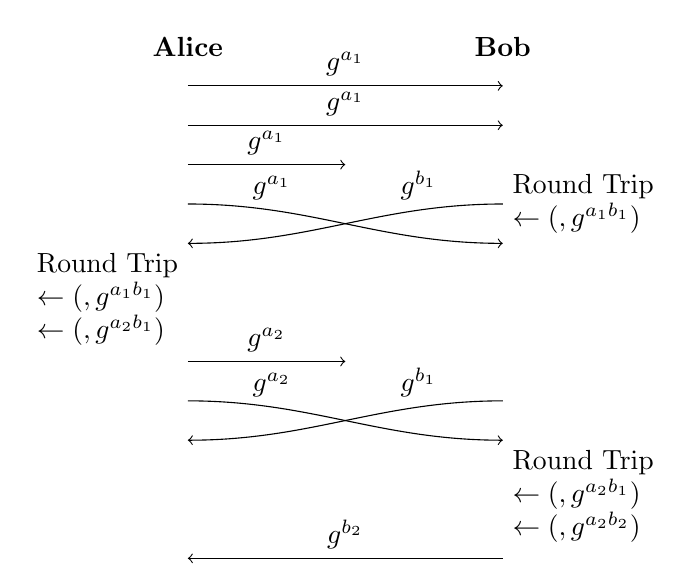
\begin{tikzpicture}
    %picture is (mostly) drawn from top to bottom depending on position of object on the left side (Alices side)
    \node (A) at (0,0) {\textbf{Alice}};
    \node (B) at (4,0) {\textbf{Bob}};
    \draw[->] (0,-.5) -- (4,-.5) node[midway,above] {$g^{a_1}$};
    \draw[->] (0,-1) -- (4,-1) node[midway,above] {$g^{a_1}$};
    \draw[->] (0,-1.5) -- (2,-1.5) node[midway,above] {$g^{a_1}$};
    %For next node: align=left to tell TikZ to align text in node left if there is a line break
    %anchor=west to place the nodes left (west) anchor at (4,-2) --> node should not be centered on (4,-2)
    \node[align=left, anchor=west] (B_RT1) at (4, -2) {Round Trip\\$\rk\gets\KDF(\rk, g^{a_1b_1})$}; 
    \draw[] (0,-2) edge[out=0, in=180, ->] node[pos=0.25, above] {$g^{a_1}$} (4,-2.5); %bend arrow with [out=0, in=180]
    %This note is anchored at north east, so the arrow points to the upper right corner 
    %(Since the node is quite high it is otherwise not clear which arrow is meant to point to it)
    \node[align=left, anchor=north east] (A_RT1) at (0, -2.5) {Round Trip\\$\rk\gets\KDF(\rk, g^{a_1b_1})$\\$\rk\gets\KDF(\rk, g^{a_2b_1})$};
    \draw[] (0, -2.5) edge[out=0, in=180, <-] node[pos=0.75, above] {$g^{b_1}$} (B_RT1);
    \draw[->] (0,-4) -- (2, -4) node[midway,above] {$g^{a_2}$};
    \node[align=left, anchor=north west] (B_RT2) at (4, -5) {Round Trip\\$\rk\gets\KDF(\rk, g^{a_2b_1})$\\$\rk\gets\KDF(\rk, g^{a_2b_2})$};
    \draw[] (0, -4.5) edge[out=0, in=180, ->] node[pos=0.25, above] {$g^{a_2}$} (4, -5);
    \draw[] (0, -5) edge[out=0, in=180, <-] node[pos=0.75, above] {$g^{b_1}$} (4, -4.5);
    \draw[<-] (0, -6.5) -- (4, -6.5) node[midway,above] {$g^{b_2}$};
\end{tikzpicture}
    \caption{An example of a simplified Double Ratchet exchange.}
    \label{fig:double-ratchet:double_ratchet}
\end{figure}

\paragraph{Asymmetric Ratchet}
The current Diffie-Hellman share is resend with every message to handle the loss of ciphertexts.
A new Diffie-Hellman key exchange~(DHKE) is performed on every full round trip.
If communication is continuous round trips will occur naturally.
Regardless, receipt acknowledgments, as are sent in many messaging protocols, amplify the frequency of completed round trips.
The asymmetric ratchet offers forward and post compromise security, as each full round trip is a full DHKE.

\paragraph{Symmetric Ratchet}
Each party maintains one ratchet for sending and one for receiving messages.
At the beginning of each round trip, the root key $\rk$ and the chain key $\ck$ are renewed with a key derivation function~(KDF): $(\rk, \ck)\gets\KDF(\rk, g^{a_i b_i})$.
The chain key is then used to derive a new chain key and a message key: $(\ck, \mk)\gets\KDF(\ck)$.

Since the message key is not used to derive new key material, it can be stored on the device until the message is sent or received.
Chain keys are deleted once the next chain key is derived.
This gives the symmetric ratchet immediate forward security.

